\chapter{Datenstrukturen}
\begin{Def}[Datenstruktur]
\hspace{\parindent}Eine Datenstruktur definiert eine Art Daten abzuspeichern, damit gewisse Operationen effizient ausgeführt werden können. Bei der Analyse betrachtet man
  \begin{itemize}
    \item die Vorverarbeitungszeit (preprocessing) um die Datenstruktur aufzubauen
    \item den Speicherplatz
    \item Zeit für die Operationen (z.B. Suchen, Einfügen, und so weiter).
  \end{itemize}
\end{Def}

Es gibt Datenstrukturen, in denen man z.B. sehr effizient suchen kann, die aber beim Einfügen oder Löschen vergleichsweise langsam sind. Andere Datenstrukturen sind darauf ausgelegt schnell Daten aufnehmen zu können, eignen sich wiederum nicht so dazu durchsucht zu werden.	

\section{Wörterbuch (dictionary)}
Als Wörterbuch versteht man einen abstrakten Datentyp, der Daten über einem Universum $\mathcal{U}$ in einer Menge $S \subseteq \mathcal{U}$  speichert. Über $\mathcal{U}$ ist meist eine lineare Ordnung definiert, z.B. $\le$.

Operationen auf Datenstrukturen, die man zu Wörterbüchern zählt sind:
\begin{itemize}
  \item \texttt{Suche}($a$, $S$): $a \in S$?
  \item \texttt{Einfügen}($a$, $S$): $S := S \cup \{a\}$
  \item \texttt{Streichen}($a$, $S$): $S := S \setminus \{a\}$
\end{itemize}

Betrachten wir uns einige konkrete Datentypen, die man als Wörterbuch ansehen kann.

\subsection{Sortiertes Feld}
Ein Sortiertes Feld ist sehr effizient, wenn es um das Suchen eines Wertes geht. Die Suche auf einem sortierten Feld lässt sich in $\mathcal{O}(\log n)$ ausführen. Für das Einfügen und Streichen von Elementen wird $\Theta(n)$ Zeit gebraucht.

\subsection{Hashing}
Unter Hashing versteht man ein Feld der Größe $m$ und eine Hashfunktion $h : \mathcal{U}\rightarrow \{ 1, \ldots, m \}$. Mit Hilfe der Hashfunktion wird die Stelle im Feld bestimmt, an der ein Element gespeichert werden soll, beziehungsweise gespeichert ist. $h$ ist im allgemeinen nicht injektiv, das heißt es kann mehrere Elemente in $S$ geben, die auf die gleiche Stelle $i$ abgebildet werden, ein entsprechendes Beispiel zeigt Abbildung \ref{kap3hashfunktion}.

\begin{figure}[htb]
  \centering
  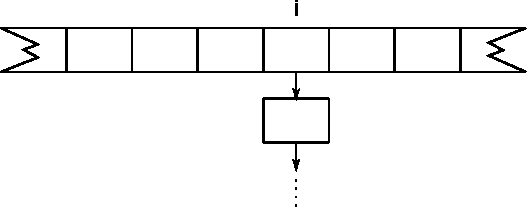
\includegraphics[scale=.8]{kap3hashfunktion}
  \caption{Die Hashfunktion ist meist nicht injektiv. Alle Elemente $x$ mit $h(x) = i$ werden in einer Liste an Stelle $i$ im Feld gespeichert.}
  \label{kap3hashfunktion}
\end{figure}

Einfügen, Suchen und Streichen kosten $\mathcal{O}(1 + \text{Länge der Liste})$ Zeit. Zumindest im Mittel $\mathcal{O}(1)$, falls es gelingt Listenlänge konstant zu halten.

Bei einem Array, wie es in Abbildung \ref{kap3hashfunktion} dargestellt wird, möchte man nicht zu viel Platz verschwenden. Entsprechende Anforderungen sind an die Hashfunktion zu stellen. Wählt man ein Element aus $\mathcal{U}$ zufällig, so sollte jede Position, die die Hashfunktion für das Element berechnet, gleich wahrscheinlich sein.

Man kann die mittlere Listenlänge auch bei beliebig vielen Einfügungen konstant halten. Sobald das Verhältnis  $\frac{|S|}{m}$ eine Konstante (zum Beispiel 2) übersteigt verdoppelt man die Anzahl der Plätze $m$ und fügt alles in das neue Feld ein. Eine einzelne Einfügung kann so zwar $\Theta(n)$ Zeit kosten, aber amortisiert über alle Einfügeoperationen erhalten wir eine Laufzeit von $\mathcal{O}(1)$.

\subsection{Binäre Suchbäume}
Ein Binärer Suchbaum ist eine Datenstruktur, bei der die Elemente in Knoten eines Baums angeordnet werden. Alle Kinder $k$ eines Knotens $a$, für die gilt $k \le a$, werden dem linken Teilbaum der Nachfolger von $a$ hinzugefügt, alle anderen Knoten dem rechten. Abbildung \ref{kap3Suchbaum} stellt das für einen Knoten und zwei Teilbäume dar.

\begin{figure}[hbt]
  \centering
  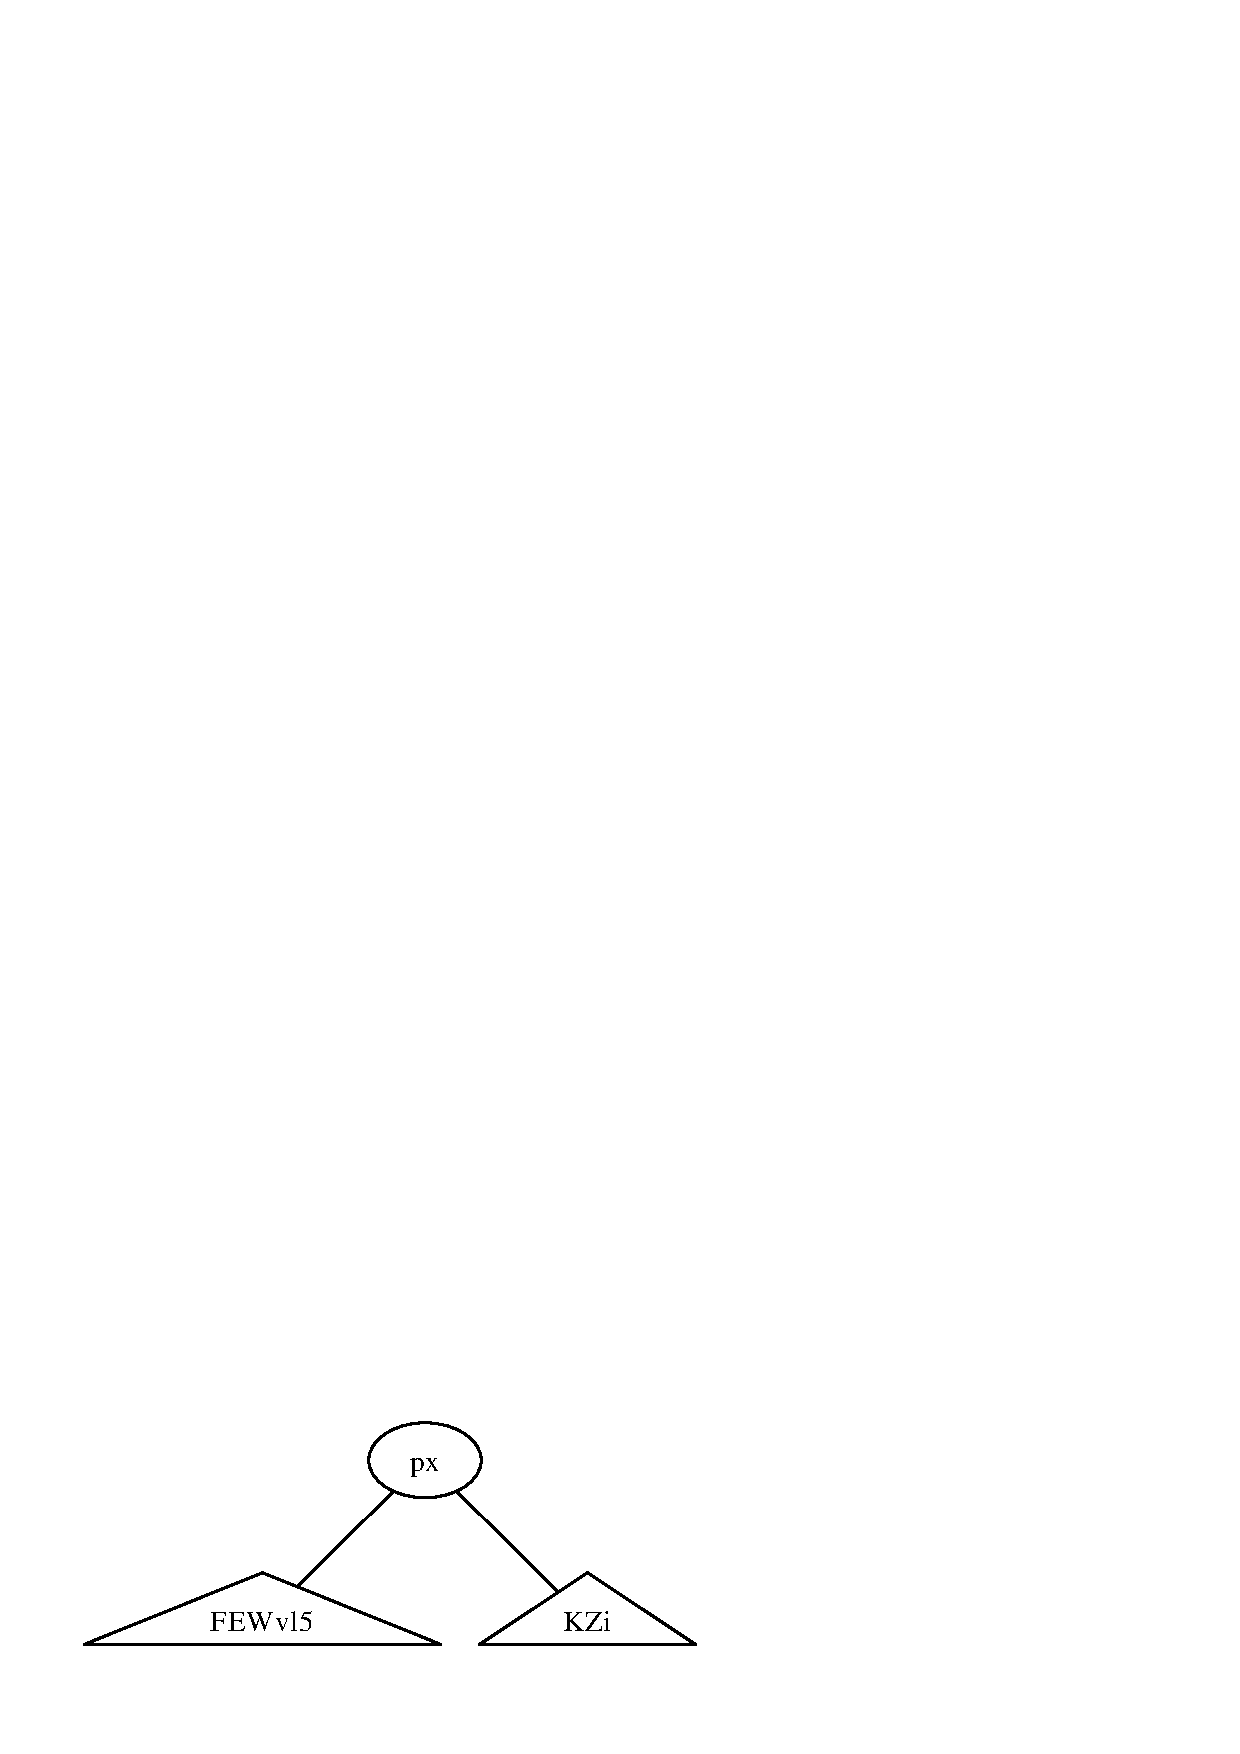
\includegraphics[scale=.75]{kap3Suchbaum}
  \caption{Jeder Knoten eines binären Suchbaums hat maximal zwei Kinder. Alle Kinder, die im linken Teilbaum angehängt sind, sind kleiner oder gleich als der Knoten $a$. Alle Kinder von $a$ die größer sind, werden zum rechten Teilbaum hinzugefügt.}
  \label{kap3Suchbaum}
\end{figure}

Die in Abbildung \ref{kap3Suchbaum} dargestellte Strukturierung gilt für jeden Teilbaum eines binären Suchbaums. Die Blätter eines binären Suchbaums enthalten keine Elemente von $S$. Jedes Blatt entspricht einer erfolglosen Suche.

Gesucht wird, in dem das gesuchte Elemente mit der Wurzel des Baums oder eines Teilbaums verglichen wird. Ist sie das gesuchte Element, kann die Suche erfolgreich beendet werden. Andernfalls wird rekursiv im linken oder rechten Teilbaum weiter gesucht, je nachdem, ob der zu vor betrachtete Knoten größer oder kleiner als das gesuchte Element war. Erreicht man ein Blatt des Baums, wird die Suche erfolglos beendet.

Zum Einfügen sucht man nach dem Element, das eingefügt werden soll, bis man ein Blatt erreicht. Anstelle des Blatts fügt man das Element ein und hängt an es zwei neue Blätter an. Beim Streichen sucht man das zu streichende Element und ersetzt es durch die Wurzel des linken Teilbaums seiner Nachfolger.

Suchen, Einfügen und Streichen von Elementen in einem binären Suchbaum lassen sich in $\mathcal{O}(h)$ Zeit realisieren, wobei $h$ für die Höhe des Baums steht. $h$ ist im günstigsten Fall (perfekt ausbalancierter Binärbaum) $\lceil \log n \rceil$ und im schlechtesten Fall (nicht ausbalancierter, entarteter Binärbaum) $n$.

Wie kann man Höhe $\mathcal{O}(\log n)$ garantieren, bei beliebigen Einfügungen und Streichungen? Dazu gibt es viele Ansätze, diese Fragestellung ist gerade in den 1970er Jahren viel untersucht worden. Wir betrachten hier zwei Methoden, die die Höhe $\mathcal{O}(\log n)$ garantieren.

\subsection{Höhenbalancierte Bäume (AVL-Bäume)}
Höhenbalancierte Bäume wurden 1962 von Addson-Velski und Landis vorgestellt, sie werden auch AVL-Bäume genannt. Höhenbalancierte Bäume sind binäre Suchbäume, wobei sich die Höhe des linken und die Höhe des rechten Teilbaums eines jeden inneren Knotens um höchstens 1 unterscheiden.

\begin{Beh}
\hspace{\parindent}Die Höhe eines AVL-Baums mit $n$ inneren Knoten ist $\Theta(\log n)$.
\end{Beh}
\begin{Bew}
\hspace{\parindent}$n_h$ sei die Mindestknotenanzahl eines AVL-Baums der Höhe $h$, also die Mindestanzahl innerer Knoten, mit der die Invariante von AVL-Bäumen erfüllt werden kann. In Abbildung \ref{kap3Mindestknotenzahl1} sehen wir drei Bäume unterschiedlicher Höhe und ihre Mindestkontenanzahl.

\begin{figure}[hbt]
  \centering
  \includegraphics[scale=0.7]{kap3Mindestknotenzahl1}
  \caption{Drei AVL-Bäume mit $n_0 = 0$, $n_1 = 1$, $n_2 = 2$.}
  \label{kap3Mindestknotenzahl1}
\end{figure}

Wir wir in Abbildung \ref{kap3Mindestknotenzahl2} sehen, lässt sich eine Rekursionsgleichung für die Mindestknotenanzahl eines AVL-Baums abhängig von seiner Höhe aufstellen:
\[ n_h = n_{h-1} + n_{h-2} + 1 \]

\begin{figure}[hbt]
  \centering
  \includegraphics[scale=0.5]{kap3Mindestknotenzahl2}
  \caption{Wenn wir die kleinste Anzahl an inneren Knoten eines AVL-Baumes betrachten, muss der linke Teilbaum $h-1$ Höhe haben, der rechte Teilbaum $h-2$.}
  \label{kap3Mindestknotenzahl2}
\end{figure}

Dies erinnert uns an die Fibonacci-Zahlen. Es gilt $n_h \ge f_{h-1}$ mit $h \ge 1$ und $f_n$ die $n$-te Fibonacci-Zahl. Wir wollen das durch Induktion beweisen. Für den Induktionsanfang mit $h=1$ und $h=2$ gilt dies, wie wir in Abbildung \ref{kap3Mindestknotenzahl1} sehen. Auch der Induktionsschritt ist einfach:
\[ n_h \quad=\quad n_{h-1} + n_{h-2} + 1 \quad\ge\quad f_{h-2} + f_{h-3} + 1 \quad=\quad f_{h-1} + 1 \quad\ge\quad f_{h-1} \qquad \surd \]

Wir wissen, dass $f_{h-1} \ge \phi^{h-2}$. Dabei ist $\phi = \frac{\sqrt{5} +1}{2}$ der sogenannte "`goldene Schnitt"'. Nun können wir $h$ besser abschätzen:
\begin{align*}
  n_h &\ge \phi^{h-2} \\
  \log n_h &\ge (h-2) \log \phi \\
  h &\le \frac{1}{\log \phi} \log n_h +2 \\
%  h &\le \underbrace{\frac{1}{\log \phi}}_{\in [1,2]} \log n_h +2 \\
  h &\le 1,44 \log n_h + 2\\
  h &= \mathcal{O}(\log n_h)\\
  &\Rightarrow \mathcal{O}(\log n) \qquad\text{mit n Anzahl der Knoten}
\end{align*}
\end{Bew}

\begin{figure}[htb]
  \centering
  \includegraphics[width=.75\textwidth]{kap3Rotation1}
  \caption{Eine Rotation hilft beim Erhalt der AVL-Eigenschaft. Der Knoten $x$ wird zur neuen Wurzel, sein rechter Teilbaum wird links an $y$ gehangen. Die Zahlen bei den Knoten geben den Wert wieder, den man erhält, wenn man die Höhe des rechten von der Höhe ihres linken Teilbaums abzieht.}
  \label{kap3Rotation1}
\end{figure}

\begin{figure}[hbt]
  \centering
  \includegraphics[width=.75\textwidth]{kap3Rotation2}
  \caption{Eine Doppelrotation kann die AVL-Eigenschaft nach dem Löschen oder Hinzufügen weiterer Elemente wieder herstellen.}
  \label{kap3Rotation2}
\end{figure}

Beim Einfügen und Streichen kann die AVL-Eigenschaft verloren gehen. Knoten, die auf dem Suchpfad vom gestrichenem oder eingefügtem Element zur Wurzel liegen, könnten außer Balance geraten. Um das zu verhindern gibt es Operationen, die die AVL-Eigenschaft wieder herstellen. In Abbildung \ref{kap3Rotation1} wird eine Rotation dargestellt, in Abbildung \ref{kap3Rotation2} eine Doppelrotation. Außerdem gibt es weitere symmetrische Fälle, diese beiden Operationen.

Jede solche Operation ist in $\mathcal{O}(1)$ Zeit durchführbar, sie müssen höchsten entlang eines Weges im Baum durchgeführt werden. Daraus folgt $\mathcal{O}(\log n)$ Zeit für die Rebalancierung, da ein Pfad höchstens diese Länge haben kann.

\begin{Satz}
\hspace{\parindent}Suchen, Einfügen und Streichen in AVL-Bäumen ist in $\mathcal{O}(\log n)$ Zeit möglich.
\end{Satz}

Ein AVL-Baum speichert die Daten, sowie jeweils noch zwei Zeiger für das rechte und das linke Kind. Ein AVL-Baum braucht somit $\mathcal{O}(n)$ Speicherplatz. Die Vorverarbeitungszeit liegt in $\mathcal{O}(n \log n)$, da das sortierte Ausgeben eines Baumes nicht besser sein kann, als $\Omega(n \log n)$ und die Ausgabe eines AVL-Baums in linearer Zeit geht.

\subsection{(a, b)-Bäume}
$(a, b)$-Bäume sind Mehrweg Suchbäume. Dabei sind $a, b \in \mathbb{N}$. Des Weiteren gilt $a \ge 2$ und $b \ge 2a -1$.

\begin{Def}
  \begin{figure}[htb]
    \centering
    \includegraphics[width=.8\textwidth]{kap3ABBaum}
  	\caption{Schematische Darstellung eines $(a,b)$-Baums, der in seinen inneren Knoten das Maximum seiner Teilbäume speichert.}
  	\label{kap3ABBaum}
  \end{figure}

\hspace{\parindent}Ein $(a, b)$-Baum ist ein Baum, in dessen Blättern die Menge $S = \{a_1, \ldots, a_n\} \subset \mathcal{U}$ mit $(\mathcal{U}, \le)$ abgelegt ist. Dabei werden folgende Bedingungen erfüllt:
\begin{itemize}
  \item alle Blätter haben gleiche Tiefe
  \item $\delta(v) \le b$ für alle Knoten v, wobei $\delta(v)$ die Anzahl der Kinder von $v$ angibt.
  \item $\delta(v) \ge a$ für alle Knoten von v
  \item $\delta(w) \ge 2$ für die Wurzel $w$
  \item Elemente von $S$ werden in den Blättern von links nach rechts aufsteigend sortiert gespeichert
  \item in jedem inneren Knoten $v$ stehen Elemente $y1 < y2 < \ldots < y_k$ mit $a-1 \le k \le b-1, k = \delta(v) -1$, so dass $y_i$ größtes Element im i-ten Unterbaum von $v$ (siehe Abbildung \ref{kap3ABBaum})
\end{itemize}
\end{Def}

\begin{figure}[htb]
  \centering
  \includegraphics[width=.8\textwidth]{kap3ABWochentage}
  \caption{Beispiel für einen $(2, 3)$-Baum, der die Wochentage enthält.}
  \label{kap3ABWochentage}
\end{figure}

Angenommen die Höhe eines $(a, b)$-Baums sei $h$. Sei $n$ die Zahl der Blätter des $(a,b)$-Baums. Wir können $n$ nun abschätzen. Die Maximale Zahl von Blättern ist $b^h$, genau dann, wenn alle inneren Knoten Grad $b$ haben. Die Minimale Zahl von Blättern ist $2\cdot a^{h-1}$, genau dann, wenn die Wurzel Grad 2 und die anderen Knoten Grad $a$ haben. Wir können also $n$ abschätzen: $2 \cdot a^{h-1} \le n \le b^h$. Daraus folgt:
\[ (h-1) \log a + 1 \le \log n \le h \log b \]
\[ (h-1) \log a       < \log n \le h \log b \]
\[ h=\mathcal{O}(\log n) \]

Betrachten wir nun die Wörterbuchoperationen auf $(a, b)$-Bäumen. Die Suche nach $a \in \mathcal{U}$ verläuft wie folgt: Vergleiche das gesuchte Element mit den Elementen $y_1, \ldots, y_k$, die in der Wurzel gespeichert sind. Ist $a \le y_1$, so wird $i=1$ gesetzt. Ist $a > y_k$, wird $i=k+1$ gesetzt. Andernfalls wird $i$ so gewählt, dass gilt $y_{i-1} < a \le y_i$. Anschließend wird der $i$-te Teilbaum rekursiv durchsucht. Der Baum muss einmal durchlaufen werden, das geschieht in $\mathcal{O}(h) = \mathcal{O}(\log n)$ Zeit.

%Suchen nach $a \in \mathcal{U}$}
%Vergleiche mit den Einträgen $y_1, \ldots, y_k$ in der Wurzel und finde $i$ mit $y_{i-1} < a \le y_i$ (bzw. $a \le y_1$, dann $i=1$ oder $a > y_k$, dann $i=k+1$). Durchsuche rekursive $i$-ten Teilbaum. $\mathcal{O}(1)$ Zeit, weil $a \le k$ und $k$ Konstante. Insgesamt $\mathcal{O}(h) = \mathcal{O}(\log n)$ Laufzeit.

Soll Element $a \in \mathcal{U}$ in einen $(a,b)$-Baum eingefügt werden, so muss die Position gefunden werden, an der ein Blatt mit Inhalt $a$ erwartet wird. Falls es nicht vorhanden ist, hängen wir ein neues Blatt mit Beschriftung $a$ an der entsprechenden Stelle an den Vaterknoten an. Hat der Vaterknoten nun $b+1$ Blätter, müssen wir ihn in zwei Knoten Spalten und überprüfen, ob der Vaterknoten des Vaterknotens dadurch zu viele Kinder hat. Dieser Vorgang setzt sich gegebenenfalls rekursiv bis zur Wurzel fort. Wird die Wurzel gespalten muss eine neue Wurzel erstellt werden, die als Kinder die Knoten enthält, die aus der Spaltung der Wurzel entstanden sind. Eine entsprechende Operation zeigt Abbildung \vref{kap3Einfuegen}.

\begin{figure}[htbp]
  \centering
  \subfloat[Es wird ein Blatt erstellt und eingefügt, der Vaterknoten hat nun jedoch mehr als $3$ Nachfolger, was in einem $(2,3)$-Baum nicht zulässig ist.]{\label{kap3EinfuegenA}\includegraphics[width=.95\textwidth]{kap3ABEinfuegenA}}
  
  \subfloat[Wir spalten den Vaterknoten und ergänzen die Wurzel um ein Element.]{\label{kap3EinfuegenB}\includegraphics[width=.95\textwidth]{kap3ABEinfuegenB}}
  
  \subfloat[Auch die Wurzel muss gespalten werden. Dazu wird eine neue Wurzel erstellt, die als Kinder die Knoten enthält, die durch die Spaltung der alten Wurzel entstanden.]{\label{kap3EinfuegenC}\includegraphics[width=.95\textwidth]{kap3ABEinfuegenC}}
  \caption{Wir fügen den fiktiven "`Etag"' (Et) in den $(2,3)$-Baum aus Abbildung \vref{kap3ABWochentage} ein.}
  \label{kap3Einfuegen}
\end{figure}

%Streichen von $a \in \mathcal{U}$
%Suchen nach a. Falls Blatt mit $a$ gefunden, entfernen wir dieses. Aktualisieren der Einträge der inneren Knoten. Ggf. Zusammenfassen von Knoten.

%Vorlesung 8

Um ein Element $a \in \mathcal{U}$ aus einem $(a,b)$-Baum zu entfernen, müssen wir das Element zu erst im Baum suchen. War die Suche erfolgreich, wird das Blatt dass $a$ enthält entfernt. Hat der Vater $v$ des Blattes nun weniger als $a$ Kinder, müssen wir weitere Operationen vornehmen, um die Invariante von $(a,b)$-Bäumen aufrecht zu erhalten. Wir unterscheiden dabei zwei Fälle:

Im ersten Fall hat der $v$ einen benachbarten Geschwisterknoten $w$, der mehr als $a$ Kinder hat. $v$ kann dann eines der äußeren Kinder von $w$ adoptieren, in die Kante zwischen dem entsprechenden Kind und $w$ gelöst und eine Kante zwischen $v$ und dem Kind erstellt wird. Anschließend sind nur noch die Beschriftungen der inneren Knoten zu aktualisieren.

Im zweiten Fall haben alle benachbarten Geschwisterknoten von $v$ nur $a$ Kinder. In diesem Fall verschmelzen wir $v$ und $w$ zu $v'$. Es kann jetzt sein, dass der Vater von $v$ und $w$ zu wenig Kinder hat und wir die Operation rekursiv fortsetzen müssen. Im schlimmsten Fall müssen wir die Kinder der Wurzel zu einer neuen Wurzel verschmelzen und die alte Wurzel entfernen. Pro Knoten braucht das konstante Zeit, insgesamt liegt die Operation damit bei $\mathcal{O}(h)$, wobei $h$ wieder die Höhe des Baumes bezeichnet. Die Operation liegt also auch in $\mathcal{O}(\log n)$.

\begin{Satz}
  \hspace{\parindent}Suchen, Einfügen, Streichen in $(a,b)$-Bäumen kostet jeweils $\mathcal{O}(\log n)$ Zeit.
\end{Satz}

\subsubsection{Amortisierte Analyse der Zahl der Spaltungen, Adoptionen und Verschmelzungen eines (a,b)-Baumes}
\begin{Beh}
  \hspace{\parindent}Werden in einem leeren $(a,b)$-Baum, mit $b \ge 2a + 1$, $n$ Einfügungen und/oder Streichungen vorgenommen, so ist die Gesamtzahl der SAV"=Operationen (Spaltungen, Adoption, Verschmelzung) höchstens $2n$. Das heißt gemittelt über alle Einfügungen und Streichungen gibt es $\mathcal{O}(1)$ SAV"=Operationen.
\end{Beh}

\begin{Bew}[mittels "`Buchhaltermethode"' (accounting method)]
  \hspace{\parindent}Für jede Einfügung/Streichung werden 2 \euro{} bezahlt. Jede SAV"=Operation kostet 1 \euro{}. Wenn am Schluss keine Schulden entstanden sind, kann es höchstens $2n$ SAV"=Operationen gegeben haben.
  
  Um das zu zeigen, gehen wir davon aus, dass jeder innere Knoten ein Konto hat, auf das das eingezahlte Geld überwiesen wird. Wir betrachten das hier Beispielhaft für einen $(2,5)$-Baum. In einem solchen Baum hat ein innerer Knoten $2, 3, 4$ oder $5$ reguläre Kinder. Beim Löschen oder Einfügen kann ein innerer Knoten vor den Operationen zum ausbalancieren des Baums auch $1$ oder $6$ Kinder haben.

  Wir stellen folgende Invariante über den Kontostand eines inneren Knotens auf:
  \begin{center}
    \begin{tabular}{l|llllll}
      Anzahl der Kinder & 1 & 2 & 3 & 4 & 5 & 6\\\hline
      Kontostand in \euro{} (mindestens) & 3 & 1 & 0 & 0 & 1 & 3
    \end{tabular}
  \end{center}
  
  Betrachten wir nun die SAV"=Operationen und überprüfen wir, ob die Invariante aufrecht erhalten werden kann. Einfüge-Operationen veranschaulicht Abbildung \vref{kap3BuchhalterA}. Streichungen veranschaulicht Abbildung \vref{kap3BuchhalterB}.

\begin{figure}[hbtp]
  \centering
  \subfloat[Einfügen eines Knotens ohne Aufspaltung erhält die Invariante Aufrecht, solange  $-1 \le c \le 2$. Da jede Einfüge"=Operation 2 \euro{} mitbringt, ist das erfüllt.]{\includegraphics{kap3BuchhalterA1}}
  
  \subfloat[Wird ein Knoten gespalten, so muss er $b+1$ Nachfolger haben. Gemäß der Invariante hat er in einem $(2,5)$-Baum also $3$ \euro{}, die beiden neuen Knoten haben je $0$ \euro{}. Von den drei Euro wird einer auf die Kosten der Operation verwendet, die beiden verbleibenden werden dem Vaterknoten gegeben, da diesem ja ein neuer Knoten hinzugefügt wird. Die Invariante bleibt also erfüllt.]{\includegraphics{kap3BuchhalterA2}}
  
  \subfloat[Muss die Wurzel gespalten werden, entstehen in einem $(2,5)$-Baum zwei neue Knoten mit je 3 Kindern, die nach der Invariante $0$ \euro{} auf dem Konto haben. Die neue Wurzel hat $2$ Kinder und braucht daher $1$ \euro{}. Das Spalten kostet $1$ \euro{}. Die alte Wurzel hatte $6$ Kinder und laut der Invariante entsprechend $3$ \euro{}. Bei der Spaltung der Wurzel ist also sogar ein Euro mehr vorhanden, als erforderlich.]{\includegraphics{kap3BuchhalterA3}}
  
  \caption{SAV"=Operationen und Invariante beim Einfügen. In den gestrichelten Kreisen wird der Kontostand der Knoten gezeigt. $c$ schätzt die Kosten der Operation ab.}
  \label{kap3BuchhalterA}
\end{figure}

\begin{figure}[hbtp]
  \centering
  \subfloat[Der Kontostand eines Knotens, dem ein Nachfolger gestrichen wird, verändert sich gemäß der Invariante um $-1 \le c \le 2$. Jede Streichung bringt $2$ \euro{} mit, so dass die Invariante erfüllt bleibt.]{\includegraphics{kap3BuchhalterB1}}
  
  \subfloat[Adoption eines Kindes: wird ein Kind von einem Knoten entfernt, da er von einem Nachbarn adoptiert wird, verändert sich der Kontostand des Knotens um $0 \le c \le 1$ \euro{}. Ein Knoten, der ein Kind adoptieren muss, hat $3$ \euro{}. Einer verbleibt bei ihm, einer deckt die Kosten der Adoption, einer steht zur Verfügung um die Änderung am Kontostand des Nachbarn auszugleichen.]{\includegraphics{kap3BuchhalterB2}}
  
  \subfloat[Verschmelzen zweier Knoten: Wir haben zwei benachbarte Knoten, einen mit einem Nachfolger, einen mit $2$ Nachfolgern. Gemäß der Invariante stehen uns also $4$ \euro{} zur Verfügung. Ein Euro wird auf die Operation an sich verwandt. Der Vaterknoten hat nun ein Kind weniger, sein Kontostand verändert sich also um $-1 \le c \le 2$ \euro{}. Selbst im schlimmsten Fall haben wir daher einen Euro mehr, als wir brauchen, um die Invariante aufrecht zu erhalten.]{\includegraphics{kap3BuchhalterB3}}
  
  \caption{SAV"=Operationen und Invariante beim Löschen. In den gestrichelten Kreisen wird der Kontostand der Knoten gezeigt.}
  \label{kap3BuchhalterB}
\end{figure}
\end{Bew}

Wir haben also für einen $(2,5)$-Baum bewiesen, dass die Anzahl der SAV"=Operationen bei $n$ Einfügungen/Streichungen $2n$ nicht übersteigt und es somit gemittelt über alle Einfügungen und Streichungen $\mathcal{O}(1)$ SAV"=Operationen gibt.

Es gibt noch andere Datenstrukturen mit $\mathcal{O}(\log n)$ für Wörterbuch Operationen.

\subsection{Rot-Schwarz-Bäume}
Rot-Schwarzbäume sind binäre Suchbäume, in denen die Knoten rot und schwarz gefärbt werden. Rot-Schwarz-Bäume weisen folgende Eigenschaften auf:
\begin{itemize}
  \item alle Blätter und die Wurzel sind schwarz
  \item rote Knoten haben 2 schwarze Kinder
  \item Jeder Weg von der Wurzel bis zu einem Blatt hat gleich viele schwarze Knoten.
\end{itemize}

\begin{figure}[htb]
  \centering
  \includegraphics[scale=.6]{kap3RSBaum}
  \caption{Beispiel: Ein Rot-Schwarz-Baum}
  \label{RSBaum}
\end{figure}

Die Höhe eines Rot"=Schwarz"=Baums liegt in $\mathcal{O}(\log n)$, wobei $n$ die Anzahl der Elemente entspricht, die der Rot-Schwarz-Baum enthalten soll. % Genau wie bei B-Bäumen sind diese in den Konten gespeichert, die Höhe eines Rot"=Schwarz"=Baums entspricht also der logarithmischen Anzahl seiner Blätter. % B-Bäume sind (a,b)-Bäume und speichern die Werte nicht in den Knoten sondern in den Blättern (im Gegensatz zu R-S-Bäumen)

Wenn man rote Knoten eines Rot"=Schwarz"=Baums mit ihren schwarzen Vätern verschmilzt, erhält man einen $(2,4)$-Baum.

\subsection{Gewichtsbalancierte Bäume}
Gewichtsbalancierte Bäume werden auch $BB[\alpha]$"=Bäume genannt. Bei $BB[\alpha]$"=Bäumen handelt es sich um binäre Suchbäume.

\begin{figure}[htb]
  \centering
  \includegraphics{kap3BBalpha}
  \caption{$balance(v) = \frac{\text{Anzahl der Blätter in } T_l}{\text{Anzahl der Blätter in } T}$}
\end{figure}

\begin{Def}[{$BB[\alpha]$-Baum}]
\hspace{\parindent}Ein $BB[\alpha]$-Baum ist ein binärer Suchbaum mit $\alpha \in (0, \frac{1}{2}]$, $balance(v) \in [\alpha, 1-\alpha]$ für jeden inneren Knoten $v$.
\end{Def}

Es gilt:
\begin{enumerate}
  \item $BB[\alpha]$-Bäume haben logarithmische Tiefe für $0 < \alpha \le \frac{1}{2}$
  \item falls $\alpha \in \left[ \frac{1}{4}, 1-\frac{\sqrt{2}}{2} \right]$ kann die $BB[\alpha]$-Eigenschaft nach Einfügungen und Streichungen durch Rotationen und Doppelrotationen wieder hergestellt werden.
\end{enumerate}

Der Beweis ist kompliziert. Wenn man das $\alpha$ zu klein macht, lässt man zu wenig Spielraum für die Rotation. Macht man $\alpha$ zu groß, kann es dazu kommen, dass man die Balance durch Rotationen und Doppelrotationen nicht wieder herstellen kann.

\subsection{Optimale Binäre Suchbäume}
\begin{Def}[optimaler binärer Suchbaum]
  \hspace{\parindent}Ein binärer Suchbaum ist optimal, wenn die erwartete Anzahl an Vergleichen für eine Suchanfrage minimal ist.
\end{Def}

Angenommen wir haben eine statische Menge $S = \{a_1, a_2, \ldots, a_n\}$ aus einem linear geordnetem Universum $(\mathcal{U}, \le)$, also $S \subseteq \mathcal{U}$. Wie sieht ein optimaler binärer Suchbaum aus? Wie sieht also ein binärer Suchbaum aus, der mit möglichst minimaler Anzahl von Vergleichen beantworten kann, ob für ein Element $a \in \mathcal{U}$ auch $a \in S$ gilt?

Für jeden inneren Knoten in einem binären Suchbaum gilt, dass die Schlüssel der Elemente seines linken Teilbaum kleiner oder gleich seines eigenen Schlüssels sind und die Elemente seines rechten Teilbaums größer seines Schlüssels sind. In den Schlüsseln der inneren Knoten speichern wir also alle Elemente der Menge $S$. Die Blätter stehen für erfolglose Suchen, also für die Intervalle zwischen den Schlüsseln in S: $(-\infty, a_1), (a_1, a_2), \ldots, (a_{n-1}, a_n), (a_n, \infty)$.

Sollten sich balancierte Bäume gut eignen, wird sich die Balance von alleine einstellen. Da $S$ statisch ist, finden keine Einfüge"= oder Streiche"=Operationen statt, wir müssen uns also keine Gedanken darüber machen, ob der Baum auszubalancieren ist oder nicht. Die Blätter können also auch unterschiedliche Tiefe haben, wenn sich das als besonders performant herausstellt.

Um zu entscheiden, welcher Knoten, wo angeordnet wird, müssen wir wissen, wie wahrscheinlich es ist, dass nach einem bestimmten Elemente aus $\mathcal{U}$ gefragt wird. Wir betrachten dazu folgende Wahrscheinlichkeiten:
\begin{enumerate}
  \item $p_i$ sei die Wahrscheinlichkeit, dass bei einer Suchanfrage nach $a_i \in S$ gefragt wird.
  \item $q_i$ sei die Wahrscheinlichkeit, dass bei einer Suchanfrage nach $a \notin S$ gefragt wird, mit $a_i < a < a_{i+1}$.
  \item $q_0$ sei die Wahrscheinlichkeit, dass nach $a$ gefragt wird, mit $a < a_1$.
  \item $q_n$ sei die Wahrscheinlichkeit, dass nach $a$ gefragt wird, mit $a > a_n$.
\end{enumerate}

Da wir es mit einer Wahrscheinlichkeitsverteilung zu tun haben gilt:
\[ \sum_{i=1}^n p_i + \sum_{j=0}^n q_j = 1\]

Wir können nun den Erwartungswert der Anzahl an Vergleichen bestimmen. Also die erwartete durchschnittliche Anzahl von Vergleichen, bei einer Anfrage an den Suchbaum. Er setzt sich zusammen aus den Zugriffswahrscheinlichkeiten für ein Element und die Anzahl der Vergleiche, die erforderlich ist, um zu bestimmen, ob das Element zur Menge $S$ gehört oder nicht:
\[ P = \sum_{i=1}^n p_i \cdot (Tiefe(i) + 1) + \sum_{i=0}^n q_i \cdot Tiefe'(i) \]
wobei $Tiefe(i)$ die Tiefe des Knotens $a_i$ angibt und $Tiefe'(i)$ die Tiefe des Blattes mit dem Schlüssel $(a_i, a_i+1)$, beziehungsweise die Tiefe des Blattes $(-\infty, a_0)$ für $i=0$ oder die Tiefe des Blattes $(a_n, \infty)$ für $i=n$. Diese Zielfunktion wollen wir minimieren, um den perfekten Suchbaum zu finden.

Die erste Summe repräsentiert die Suche nach einem Element $a_i \in S$. Sie summiert für alle Elemente aus $S$ das Produkt aus Anfragewahrscheinlichkeit des Elements und die Anzahl der nötigen Vergleichsoperationen zum Finden des repräsentierenden Knotens. Die Anzahl der Verlgeichsoperationen entspricht der Tiefe des Knotens $+1$ für den Vergleich mit der Wurzel.

Die zweite Summe summiert über die übrigen Anfragen. Das sind Anfragen nach Elementen, die nicht in $S$ gespeichert sind. Alle diese Elemente liegen in den Intervallen, die in als Schlüssel der Blätter genutzt werden. Wir können, um die Anzahl der Vergleiche zu ermitteln, also die Zugriffswahrscheinlichkeit auf eines dieser Elemente mit der Tiefe des Blatts multiplizieren, welches das Intervall enthält, in dem das gesuchte Element liegt.

\subsubsection{Drei beispielhafte Suchbäume}


Betrachten wir ein Beispiel. Sei $\mathcal{U} = \{1, 2, 3, 4, 5, 6, 7\}$ und $S = \{2, 5, 6\}$. Nach den Elementen aus $S$ wird mit den Wahrscheinlichkeiten $p_1 = 0{,}3,\quad p_2 = 0{,}2,\quad p_3 = 0{,}1$ gefragt. Die Intervalle zwischen den Elementen in $S$ seien gleich wahrscheinlich, d.h. $q_0 = q_1 = q_2 = q_3 = 0{,}1$. In Abbildung \vref{kap3OptimaleSB} sehen wir drei mögliche Suchbäume.

\begin{figure}[htb]
  \centering
  \subfloat[Baum $T_1$\label{kap3OptimaleSBT1}]{\includegraphics[width=.4\textwidth]{kap3OptimaleSB2}}
  
  \subfloat[Baum $T_2$\label{kap3OptimaleSBT2}]{\includegraphics[width=.3\textwidth]{kap3OptimaleSB1}}\hspace{.05\textwidth}
  \subfloat[Baum $T_3$\label{kap3OptimaleSBT3}]{\includegraphics[width=.3\textwidth]{kap3OptimaleSB3}}

  \caption{Drei mögliche Suchbäume über die Elemente $S=\{a_1, a_2, a_3\}$ mit bekannter Zugriffswahrscheinlichkeit $0{,}1 - 0{,}3$.}
  \label{kap3OptimaleSB}
\end{figure}

Die erwartete durchschnittliche Suchzeit (Zahl der Vergleiche) für die in Abbildung \vref{kap3OptimaleSB} dargestellten Suchbäume ist:
\begin{align*}
  P_{T_1} &= (0{,}2 + 0{,}3 \cdot 2 + 0{,}1 \cdot 2) + (2 \cdot 0{,}1 + 2 \cdot 0{,}1 + 2 \cdot 0{,}1 + 2 \cdot 0{,}1)\\
          &= 1{,}8\\
  P_{T_2} &= (0{,}1 + 0{,}2 \cdot 2 + 0{,}3 \cdot 3) + (0{,}1 + 0{,}1 \cdot 2 + 0{,}1 \cdot 3 + 0{,}1 \cdot 3)\\
          &= 2{,}3\\
  P_{T_3} &= (0{,}3 + 0{,}2 \cdot 2 + 0{,}1 \cdot 3) + (0{,}1 + 0{,}1 \cdot 2 + 0{,}1 \cdot 3 + 0{,}1 \cdot 3)\\
          &= 1{,}9\\
\end{align*}

In diesem Beispiel, ist also der Baum $T_1$ besser, als die Bäume $T_2$ oder $T_3$.

\subsubsection{Optimale BST und dynamische Programmierung}
Per \textit{brute force} alle möglichen Suchbäume zu erzeugen und zu untersuchen, lässt sich jedoch nur für sehr kleine $|S|=n$ durchführen. Es gibt $\binom{2n}{n} \cdot \frac{1}{n+1} \approx 4^n$ mögliche Suchbäume, das heißt bereits bei $n=5$ wären über $1.000$ Bäume zu untersuchen. Mit der Methode des \textit{dynamischen Programmierens} können wir das Problem jedoch effizienter lösen. 

\textit{Dynamische Programmierung} bietet sich an, wenn sich ein Problem in kleinere Teilprobleme zerlegen lässt, die sich wiederum in kleinere Teilprobleme zerlegen lassen. Die kleinste Einheit dieser Teilprobleme wird gelöst, die Lösung gespeichert, so dass sie für die Lösung verschiedener größerer Teilprobleme genutzt werden kann, ohne jedes mal neu bestimmt zu werden. Jedes Teilproblem muss so nur einmal gelöst werden, auch wenn es zum Gesamtproblem mehrfach beiträgt.

Versuchen wir nun die Suche nach einem optimalen binären Suchbaum in solche Teilprobleme aufzuteilen:
\begin{itemize}
  \item Sei $S'=\{a_i, \ldots, a_j\}$ eine Teilmenge  der Menge $S$, also $S' \subset S$.
  \item Mit $T_{i,j}$ bezeichnen wir den optimalen Suchbaum für $S'$.
  \item Die Wurzel von $T_{i,j}$ sei $a_m$, $m \in \{i, \ldots, j\}$.
  \item Die inneren Knoten von $T_{i,j}$ sind $\{a_i, \ldots, a_j\}$.
  \item Wir speichern $(a_{i-1}, a_i), (a_i, a_{i+1}) \ldots, (a_{j-1}, a_j), (a_j, a_{j+1})$ in den Blättern von $T_{i,j}$, also genau wie bei $S$ die Intervalle über die Bereiche vor, zwischen und nach den gespeicherten Elementen.
  \item Mit $P_{T_{i,j}}$ bezeichnen wir die erwartete durchschnittliche Anzahl an Vergleichen, um zu bestimmen, ob ein Element im Teilbaum $T_{i,j}$ gespeichert ist, oder nicht, unter der Bedingung, dass wir die Suche bereits auf den Teilbaum eingeschränkt haben.
  \item Die Zugriffswahrscheinlichkeiten auf Elemente des Teilbaums (die in den inneren Knoten gespeichert werden) geben wir mit $\widetilde{p_i} = \frac{p_i}{w_{i,j}}$ an, die Zugriffswahrscheinlichkeiten auf seine Blätter mit $\widetilde{q_i} = \frac{q_i}{w_{i,j}}$ an. Dabei bezeichnet $w_{i,j}$ die Wahrscheinlichkeit, dass nach einem Element $a \in [a_i, a_j]$ gesucht wird, also $w_{i,j} = p_i + \ldots + p_j + q_{i-1} + q_i + \ldots + q_j$. $\widetilde{p_i}$ und $\widetilde{q_i}$ sind also bedingte Wahrscheinlichkeiten.\footnote{$P(A|B)=\frac{P(A \cap B)}{P(B)}$ und wenn $A \subset B$, dann $P(A|B) = \frac{P(A)}{P(B)}$.}
\end{itemize}

\begin{figure}[hbt]
  \centering
  \includegraphics[width=.5\textwidth]{kap3SucheOSB}
  \caption{Die Suche eines optimalen Suchbaums lässt sich in Teilprobleme aufspalten. Darstellung zur Veranschaulichung der Bezeichnungen der Teilbäume und wichtiger Knoten.}
  \label{kap3SucheOSB}
\end{figure}

Wir wissen, dass sich $T_{i,j}$ aus $a_m$ und zwei Teilbäumen zusammensetzt: $T_{i, m-1}$ und $T_{m+1,j}$. Abbildung \ref{kap3SucheOSB} veranschaulicht das. Dies nutzen wir um die erwartetet Anzahl von Vergleichen in $T_{i,j}$ zu bestimmen. Zu beachten ist, dass $\widetilde{p_i}=\frac{p_i}{w_{i,j}}$ und $\widetilde{q_i}=\frac{q_i}{w_{i,j}}$ gilt.
\begin{align*}
P_{T_{i,j}} &= \sum_{k=i}^{j} \widetilde{p_k} \cdot (Tiefe(k) + 1) + \sum_{k=i-1}^{j} \widetilde{q_k} \cdot Tiefe'(k) \\
	&= \frac{1}{w_{i,j}} \cdot \left( \sum_{k=i}^{j} p_k \cdot (Tiefe(k) + 1) + \sum_{k=i-1}^{j} q_k \cdot Tiefe'(k) \right)\\
	&= \frac{1}{w_{i,j}} \cdot \left( \sum_{k=i}^{m-1} p_k \cdot (Tiefe(k) + 1) + p_m + \sum_{k=m+1}^{j} p_k \cdot (Tiefe(k) + 1)\right. \\
	& \phantom{= \frac{1}{w_{i,j}}} \quad \left. + \sum_{k=i-1}^{m-1} q_k \cdot Tiefe'(k) + \sum_{k=m}^{j} q_k \cdot Tiefe'(k)\right)
\end{align*}
Wenn wir hier die Summen durch die Formeln für die Teilbäume ersetzen müssen wir zwei Dinge berücksichtigen. $P_{T_{i,m-1}}$ berechnet die bedingte Wahrscheinlichkeit, bedingt darauf, dass wir nach einem Knoten in dem Teilbaum $T_{i,m-1}$ gefragt werden. Wir wissen bereits, dass wir in dem Teilbaum sind, müssen daher $P_{T_{i,m-1}}$ mit $w_{i,m-1}$ multiplizieren. Die Formel für $P_{T_{i,m-1}}$ berücksichtigt die Tiefe eines Knotens, bzw. die Tiefe eines Blattes. Von $P_{T_{i,m-1}}$ aus betrachtet ist die Tiefe jedoch um $1$ geringer, als von $P_{T_{i,j}}$ aus betrachtet.
\begin{align*}
  P_{T_{i,j}} &= \frac{1}{w_{i,j}} \cdot \left( \sum_{k=i}^{m-1} p_k \cdot (Tiefe(k) + 1) + \sum_{k=i-1}^{m-1} q_k \cdot Tiefe'(k) + p_m \right.\\
    & \phantom{= \frac{1}{w_{i,j}}} \quad \left. + \sum_{k=m+1}^{j} p_k \cdot (Tiefe(k) + 1) + \sum_{k=m}^{j} q_k \cdot Tiefe'(k) \right)\\
    &= \frac{ w_{i,m-1} \cdot P_{T_{i,m-1}} +  w_{i,m-1} + p_m + w_{m+1, j} + w_{m+1,j} \cdot P_{T_m+1, j} }{w_{i,j}}\\
    &= 1 + \frac{w_{i,m-1} \cdot P_{T_{i,m-1}} + w_{m+1, j} \cdot P_{T_{m+1,j}}}{w_{i,j}}
\end{align*}

%\[ P_{T_{i,j}} = \sum_{k=i}^{j} \widetilde{p_k} \cdot (Tiefe(k) + 1) + \sum_{k=i-1}^{j} \widetilde{q_k} \cdot Tiefe'(k) \]
%Wir lösen nun $\widetilde{p_k}$ und $\widetilde{q_k}$ auf, da $\widetilde{p_i}=\frac{p_i}{w_{i,j}}$ und $\widetilde{q_i}=\frac{q_i}{w_{i,j}}$.
%\[ P_{T_{i,j}} = \frac{1}{w_{i,j}} \cdot \left( \sum_{k=i}^{j} p_k \cdot (Tiefe(k) + 1) + \sum_{k=i-1}^{j} q_k \cdot Tiefe'(k) \right) \]
%Wir teilen die Summenformeln neu auf, wobei wir beachten, dass $Tiefe(m) = 0$, weil $a_m$ die Wurzel von $T_{i,j}$ ist.
%\[ \sum_{k=i}^{j} p_k \cdot (Tiefe(k) + 1) = \sum_{k=i}^{m-1} p_k \cdot (Tiefe(k) + 1) + p_m + \sum_{k=m+1}^{j} p_k \cdot (Tiefe(k) + 1) \]
%Analog gilt:
%\[ \sum_{k=i-1}^{j} q_k \cdot Tiefe'(k) = \sum_{k=i-1}^{m-1} q_k \cdot Tiefe'(k) + \sum_{k=m}^{j} q_k \cdot Tiefe'(k) \]
%Wir können nun die Formel für den Teilbaum $T_{i, m-1}$ aufstellen:
%\[ P_{T_{i,m-1}} = \sum_{k=i}^{m-1} \widehat{p_k} \cdot (Tiefe(k) + 1) + \sum_{k=i-1}^{m-1} \widehat{q_k} \cdot Tiefe'(k)\]
%wobei natürlich $\widehat{p_k} = \frac{p_k}{w_{i,m-1}}$ und $\widehat{q_k} = \frac{q_k}{w_{i,m-1}}$. Genauso lässt sich die Formel für den Teilbaum $T_{m+1,j}$ aufstellen:
%\[ P_{T_{m+1, }} = \sum_{k=m+1}^{j} \overline{p_k} \cdot (Tiefe(k) + 1) + \sum_{k=m}^{j} \overline{q_k} \cdot Tiefe'(k) \]
%natürlich mit $\overline{p_k} = \frac{p_k}{w_{m+1, j}}$ und $\overline{q_k} = \frac{q_k}{w_{m+1, j}}$. Wenn wir das zu einer Formel zusammenfassen, müssen wir beachten, dass wir nicht mehrfach berücksichtigen, die Suche bereits auf einen Teilbaum beschränkt zu haben. Wir müssen daher $P_{T_{i,m-1}}$ mit $w_{i,m-1}$ multiplizieren und $P_{T_{m+1,j}}$ mit $w_{m+1, j}$.
%
%Wir können das nun zu einer neuen Formel für $P_{T_{i,j}}$ zusammenfassen:
%\[ P_{T_{i,j}} = \frac{w_{i,m-1} \cdot P_{T_{i,m-1}} + p_m + w_{m+1, j} \cdot P_{T_{m+1,j}}}{w_{i,j}} \]

%\begin{align*}
%  P_{T_{i,j}} &= \sum_{k=i}^{j} \widetilde{p_k} \cdot (Tiefe(k) + 1) + \sum_{k=i-1}^{j} \widetilde{q_k} \cdot Tiefe'(k)\\
%    &= \sum_{k=i}^{j} \frac{p_k}{w_{i,j}} \cdot (Tiefe(k) + 1) + \sum_{k=i-1}^{j} \frac{q_k}{w_{i,j}} \cdot Tiefe'(k)\\
%  w_{i,j} \cdot P_{T_{i,j}} &= \sum_{k=i}^{j} p_k \cdot (Tiefe(k) + 1) + \sum_{k=i-1}^{j} q_k \cdot Tiefe'(k)\\
%    &= \sum_{k=i}^{j} \left[ p_k \cdot (Tiefe(k) + 1) + q_k \cdot Tiefe'(k) \right] + q_{i-1} \cdot Tiefe'(i-1) \\
%    &= \sum_{k=i}^{m-1} \left[ p_k \cdot (Tiefe(k) + 1) + q_k \cdot Tiefe'(k) \right] \\
%    &\qquad + p_m \cdot (\underbrace{Tiefe(m)}_{=0} +1 ) + q_m \cdot Tiefe'(m) \\
%    &\qquad + \sum_{k=m+1}^j \left[ p_k \cdot (Tiefe(k) + 1) + q_k \cdot Tiefe'(k) \right] \\
%    &\qquad + q_{i-1} \cdot Tiefe'(i-1)\\
%    &= \sum_{k=i}^{m-1} \left[ w_{i,m-1} \cdot \frac{p_k}{w_{i,m-1}} \cdot (Tiefe(k) + 1) +  w_{i,m-1} \cdot \frac{q_k}{w_{i,m-1}} \cdot Tiefe'(k) \right] \\
%        &\qquad + p_m + q_m \cdot Tiefe'(m) + q_{i-1} \cdot Tiefe'(i-1)\\
%        &\qquad + \sum_{k=m+1}^j \left[ w_{m+1,j} \cdot \frac{p_k}{w_{m+1,j}} \cdot (Tiefe(k) + 1) + w_{m+1,j} \cdot \frac{q_k}{w_{m+1,j}} \cdot Tiefe'(k) \right] \\
%    &=  w_{i,m-1} \cdot \sum_{k=i}^{m-1} \left[\widehat{p_k} \cdot (Tiefe(k) + 1) + \widehat{q_k} \cdot Tiefe'(k) \right] \\
%            &\qquad + p_m + q_m \cdot Tiefe'(m) + q_{i-1} \cdot Tiefe'(i-1)\\
%            &\qquad + w_{m+1,j} \sum_{k=m+1}^j \left[ \overline{p_k} \cdot (Tiefe(k) + 1) + \overline{q_k} \cdot Tiefe'(k) \right] \\
%    &=  w_{i,m-1} \cdot P_{T_{i, m-1}} - q_{i-1} \cdot Tiefe'(i-1) \\
%    &\qquad +  p_m + q_m \cdot Tiefe'(m)  + q_{i-1} \cdot Tiefe'(i-1) \\
%    &\qquad + w_{m+1,j} \cdot P_{T_{m+1, j}} - q_m \cdot (Tiefe'(m)) \\
%    &= w_{i,m-1} \cdot P_{T_{i, m-1}} + p_m + w_{m+1,j} \cdot P_{T_{m+1, j}}\\
%    P_{T_{i,j}} &= \frac{w_{i,m-1} \cdot P_{T_{i, m-1}} + p_m + w_{m+1,j} \cdot P_{T_{m+1, j}}}{w_{i,j}}\\
%                &= 1 + \frac{w_{i,m-1} \cdot P_{T_{i, m-1}} + w_{m+1,j} \cdot P_{T_{m+1, j}}}{w_{i,j}}
%\end{align*}
%
%Daraus folgt:
%\[ P_{T_{i,j}} = 1 + \frac{w_{i,m-1} \cdot P_{T_{i,m-1}} + w_{m+1, j} \cdot P_{T_{m+1,j}}}{w_{i,j}} \]

\begin{Lma}
  \hspace{\parindent}Der Teilbaum $T_{i,j}$ sei ein optimaler binärer Suchbaum für die Menge $\{a_i, \ldots, a_j\}$. $a_m$ sei die Wurzel von $T_{i,j}$, $T_{i,m-1}$ der linke und $T_{m+1,j}$ der rechte Teilbaum von $T_{i,j}$. Dann ist $T_{i,m-1}$ der optimale binäre Suchbaum für die Menge $\{a_i, \ldots, a_{m-1}\}$ und $T_{m+1,j}$ der optimale binäre Suchbaum der Menge $\{a_{m+1}, \ldots, a_j\}$.
\end{Lma}

\begin{Bew}
  \hspace{\parindent}Angenommen es existiert ein Baum $T'_{i,m-1}$ mit $P_{T'_{i,m-1}} < P_{T_{i,m-1}}$. Dann wäre auch $P_{T'_{i,j}} < P_{T_{i,j}}$, da:
  \begin{align*}
    P_{T'_{i,j}} &= 1 + \frac{w_{i,m-1} \cdot P_{T'_{i,m-1}} + w_{m+1, j} \cdot P_{T_{m+1,j}}}{w_{i,j}}\\
      &< 1 + \frac{w_{i,m-1} \cdot P_{T_{i,m-1}} + w_{m+1, j} \cdot P_{T_{m+1,j}}}{w_{i,j}} = P_{T_{i,j}}
  \end{align*}
  dies steht aber in Widerspruch dazu, dass $P_{T_{i,j}}$ ein optimaler binärer Suchbaum ist. Jeder Teilbaum von $P_{T_{i,j}}$ muss daher selber ein optimaler binärer Suchbaum sein.
\end{Bew}

Wir haben nun alles zusammen um mit Hilfe der Methode des dynamischen Programmierens einen Algorithmus zum Finden eines optimalen binären Suchbaums anzugeben.
Wir vereinbaren folgende Variablen für den Algorithmus:
\begin{align*}
  r_{i,j} &:= \text{Index der Wurzel von } T_{i,j}\\
  c_{i,j} &:= w_{i,j} \cdot P_{T_{i,j}} = \text{ Kosten von } T_{i,j}\\
  w_{i,j} &:= \text{Wahrscheinlichkeit, dass } a \in \{a_i, \ldots, a_j\}
\end{align*}

Es ist leicht zu erkennen, dass $w_{i,j} = w_{i, m-1} + p_m + w_{m+1, j}$ gilt. Man kann $c_{i,j}$ auch rekursiv berechnen. $c_{i,j}$ setzt sich aus den Kosten seiner Teilbäume zusammen, die Tiefe der Knoten in den Teilbäumen ist jedoch um eins erhöht. Daher gilt: $c_{i,j} = c_{i,m-1} + p_m + c_{m+1,j} + w_{i,m-1} + w_{m+1,j} = w_{i,j} + c_{i,m-1} + c_{m+1, j}$. Für $i=m$ gibt es keinen linken Teilbaum, für $m=j$ gibt es keinen rechten Teilbaum. $T_{i,i}$ definieren wir als leeren Baum, mit dem Gewicht $w_{i,i} = q_i$ und den Kosten $c_{i,i}=0$.

% Algorithmus aus dem Vorlesungsskript
\begin{Alg}[Finden eines optimalen binären Suchbaums]
\begin{algorithmic}[1]
  \Function{Finde Baum}{$p_1, \ldots, p_n$, $q_0, \ldots, q_n$}
    \For{$i = 0, \ldots, n$}
      \State $w_{i+1,i} = q_i$
      \State $c_{i+1,i} = 0$
    \EndFor
    \For{$k=0, \ldots, n-1$}
      \For{$i=1, \ldots, n-k$}
        \State $j=i+k$
        \State Bestimme $m$ mit $i \le m \le j$, so dass $c_{i,m-1} + c_{m+1,j}$ minimal ist.
        \State $r_{i,j} = m$
        \State $w_{i,j} = w_{i,m-1} + p_m + w_{m+1, j}$
        \State $c_{i,j} = c_{i, m-1} + c_{m+1, j} + w_{i, j}$
      \EndFor
    \EndFor
  \EndFunction
\end{algorithmic}
\end{Alg}

% Aho, Hopcroft, Ullman: The Design an Analysis of Computer Algorithms
%\begin{Alg}[Finden eines optimalen binären Suchbaums]
%\begin{algorithmic}[1]
%  \For{$i = 0, \ldots, n$}
%    \State $w_{i,i} = q_i$
%    \State $c_{i,i} = 0$
%  \EndFor
%  \For{$k=1, \ldots n$}
%    \For{$i=0, \ldots, n-k$}
%      \State $j=i+k$
%      \State Bestimme $m$ mit $i < m \le j$, so dass $c_{i,m-1} + c_{m+1,j}$ minimal ist.
%      \State $r_{i,j} = m$
%      \State $w_{i,j} = w_{i,m-1} + p_m + w_{m+1, j}$
%      \State $c_{i,j} = c_{i, m-1} + c_{m+1, j} + w_{i, j}$
%    \EndFor
%  \EndFor
%\end{algorithmic}
%\end{Alg}

Der Algorithmus basiert auf einem von Richard Bellman 1957 gefundenen Satz über optimale mittlere Suchdauer in binären Suchbäumen. Die Teilprobleme, in die die Suche nach dem optimalen binären Suchbaum aufgeteilt wird, sind die Teilbäume $T_i,j$. Der Algorithmus sucht für jeden dieser Teilbäume die optimale Wurzel, bestimmt das Gewicht des Teilbaums und die Kosten für die Suche im Teilbaum. Diese Werte werden dann genutzt, um größere Teilbäume zu berechnen. Als Ergebnis bekommen wir die Wurzeln aller Teilbäume, angefangen bei Teilbäumen, die lediglich einen Knoten enthalten, bis zum gesuchten Teilbaum $T_{1,n}$.

\subsubsection{Beispielhafte Suche nach dem optimalen binären Suchbaum}
Wer veranschaulichen das Vorgehen des Algorithmus, in dem wir das Beispiel von oben nachvollziehen. $S$ ist demnach die Menge $\{2, 5, 6\}$ mit den Zugriffswahrscheinlichkeiten $p_1 = 0{,}3,\quad p_2 = 0{,}2,\quad p_3 = 0{,} 1$ und $q_0 = q_1 = q_2 = q_3 = 0{,}1$. Der Algorithmus erzeugt dann folgende Tabelle:

\begin{center}
\begin{tabular}{|>{$}c<{$}||>{$}c<{$}|>{$}c<{$}|>{$}c<{$}|>{$}c<{$}|>{$}c<{$}|}\hline
 & i=0 & i=1 & i=2 & i=3 \\\hline\hline
\multirow{2}*{Init} & w_{1,0}=0{,}1 & w_{2,1} = 0{,}1 & w_{3,2}= 0{,}1 & w_{4,3} = 0{,}1 \\
                    & c_{1,0}=0\hphantom{0} & c_{2,1} = 0\hphantom{0} & c_{3,2}=0\hphantom{0} & c_{4,3}=0\hphantom{0}\\\hline
\multirow{3}*{k=0}  & & r_{1,1}=1\hphantom{0} & r_{2,2}=2\hphantom{0} & r_{3,3}=3\hphantom{0} \\
                    & & w_{1,1}=0{,}5 & w_{2,2}=0{,}4 & w_{3,3}=0{,}3\\
                    & & c_{1,1}=0{,}5 & c_{2,2}=0{,}4 & c_{3,3}=0{,}3\\\hline
\multirow{3}*{k=1}  & & r_{1,2}=1\hphantom{0}& r_{2,3}=2\hphantom{0}& \\
                    & & w_{1,2}=0{,}8 & w_{2,3}=0{,}6 & \\
                    & & c_{1,2}=1{,}2 & c_{2,3}=0{,}9 & \\\hline
\multirow{3}*{k=2}  & & r_{1,3}=2\hphantom{0}& & \\
                    & & w_{1,3}=1{,}0 & & \\
                    & & c_{1,3}=1{,}8 & & \\\hline
\end{tabular}
\end{center}

Aus dieser Tabelle lässt sich nun leicht der optimale binäre Suchbaum erstellen.
\begin{Alg}
\begin{algorithmic}[1]
  \Procedure{Erzeuge Baum}{$i$, $j$}
    \State Erzeuge Knoten $v_{i,j}$ als Wurzel von $T_{i,j}$.
    \State Knoten $v_{i,j}$ wird dabei mit $s_{r_{i,j}}, \text{ mit } s \in S$ beschriftet.
    \If{$i < r_{i,j}$}
      \State \textsc{Erzeuge Baum}($i$, $r_{i,j}-1$) als linken Teilbaum von $v_{i,j}$
    \EndIf
    \If{$r_{i,j} < j$}
      \State \textsc{Erzeuge Baum}($r_{i,j} + 1$, $j$) als rechten Teilbaum von $v_{i,j}$
    \EndIf
  \EndProcedure
\end{algorithmic}
\end{Alg}

Wir beginnen  mit \textsc{Erzeuge Baum($1, 3$)}. Die Wurzel $v_{1,3}$ ist $a_2$. Um den linken Teilbaum zu erzeugen rufen wir \textsc{Erzeuge Baum($1, 1$)} auf und finden $v_{1,1} = a_1$. Um den rechten Teilbaum zu erzeugen rufen wir \textsc{Erzeuge Baum($3, 3$)} auf und finden die Wurzel $v_{3,3} = a_2$. Anschließend erzeugen wir die Blätter, per Definition als Intervalle. Wir erhalten so den Baum, den wir bereits in Abbildung \vref{kap3OptimaleSBT1} gesehen haben.

\subsubsection{Analyse von Laufzeit und Speicherverhalten}
Der Algorithmus muss die Zwischenergebnisse speichern. Eine Tabelle, wie wir sie oben genutzt haben können wir als Matrix $M \in \mathcal{M}((n + 1) \times n, \mathbb{R})$ auffassen. Der Speicherplatz beträgt also $S(n) = n \cdot (n+1) = n^2 + n \in \mathcal{O}(n^2)$.

Betrachten wir das Laufzeitverhalten des Algorithmus. Die Zeilen 2 bis 5 können wir mit $c_1 \cdot (n+1)$ ansetzen. Zeile 8 ist eine einfache Operation konstanter Zeit, im folgenden mit $c_2$ berücksichtigt. In Zeile 9 müssen wir $(j-i) = k$ zuvor berechnete Werte nachschauen und vergleichen. Dafür berechnen wir $k \cdot c_3$. Zeile 10 bis 12 brauchen wieder konstante Zeit, also $c_4$. Daher:
\[ T(n) = c_1 \cdot n + c_1 + \sum_{k=0}^{n-1} \sum_{i=1}^{n-k} \left( c_2 + k \cdot c_3 + c_4\right) \]
$c_2 + c_4$ fassen wir zu $c_5$ zusammen:
\begin{align*}
  T(n) &= c_1 \cdot n + c_1 + \sum_{k=0}^{n-1} \sum_{i=1}^{n-k} \left( c_5 + k \cdot c_3 \right)\\
       &= c_1 \cdot n + c_1 + \sum_{k=0}^{n-1} \left( (n-k) \cdot c_5 + (n-k) \cdot k \cdot c_3 \right)\\
       &= c_1 \cdot n + c_1 + c_5 \cdot \sum_{k=0}^{n-1} (n-k) + c_3 \cdot \sum_{k=0}^{n-1} (nk - k^2)\\
       &= c_1 \cdot n + c_1 + c_5 \cdot \sum_{k=1}^{n} k + c_3 \cdot \left( n \cdot \sum_{k=1}^{n-1} k - \sum_{k=1}^{n-1} k^2\right)\\
       &= c_1 \cdot n + c_1 + c_5 \cdot \frac{n^2 + n}{2} + c_3 \cdot \left( n \cdot \left( \frac{n^2 + n}{2} -n \right) - \frac{2n^3 + 3n^2 + n}{6} -n^2 \right)\\
       &= c_1 \cdot n + c_1 + c_5 \cdot \frac{n^2 + n}{2} + c_3 \cdot \left( \frac{n^3 - n}{6} \right)\\
       &\in \mathcal{O}(n) + \mathcal{O}(n^2) + \mathcal{O}(n^3)
\end{align*}
Der Algorithmus liegt also in $\mathcal{O}(n^3)$.

\subsubsection{Optimierung}
Durch die dynamische Programmierung hat der Algorithmus mindestens quadratische Laufzeit. Die kubische Laufzeit des Algorithmus beruht auf einer Kombination des dynamischen Programmierens und der Suche nach der Wurzel in Zeile 9 des Algorithmus. Donald E. Knuth hat in seinem Buch \textit{The Art of Computer Programming} Band 3: \textit{Sorting and Searching.} folgendes Lemma bewiesen:

\begin{Lma}
  \hspace{\parindent}$r_{i,j-1} \le r_{i,j} \le r_{i+1, j}$.
\end{Lma}

Durch die Eingrenzung der Wurzelsuche durch das Lemma, kann die Laufzeit des Algorithmus auf $T(n) \in \mathcal{O}(n^2)$ reduziert werden.

% vorlesung 10
\subsection{Sonstige Datenstrukturen für das Wörterbuchproblem}
Binäre Suchbäume weißen in schlechten Fällen, schlechte Laufzeiten bei der Suche auf. Als Antwort darauf haben wir uns balancierte Bäume angeschaut, z.B. AVL-Bäume oder $(a,b)$-Bäume, die oft als B-Bäume bezeichnet werden. Es gibt noch mehr Bäume mit verschiedenen Vorschriften. Wir haben uns schließlich optimale binäre Suchbäume angeschaut. Oft kennt man die Wahrscheinlichkeiten nicht, wie oft man nach welchen Daten gefragt wird, kann also keinen optimalen Suchbaum aufbauen.

Es gibt weitere Datenstrukturen für das Wörterbuchproblem. Einige arbeiten zum Beispiel mit einer Move"=To"=Front"=Heuristik. Dabei werden die Daten, nach denen gefragt wird, so verschoben, dass sie schneller zu finden sind, als Daten, nach denen lange nicht mehr gefragt wurden (z.B. an den Anfang einer Liste oder eines Arrays). Ein solche Vorgehen lässt sich auch auf Bäumen implementieren: Splay-Trees sind selbstorganisierende Suchbäume. Die Daten, auf die zugegriffen wird, werden durch Rotation und Doppelrotation innerhalb des Baums "`nach oben"' bewegt.

Für spezielle Datenmengen lassen sich noch bessere Datenstrukturen entwickeln. Ein \textit{Trie} ist ein digitaler Suchbaum, der zum Beispiel gerne von Suchmaschinen im Internet, von Programmen zur Textverarbeitung oder in der Bioinformatik zur Speicherung von DNA"=Folgen genutzt wird.

\begin{figure}[hbt]
  \centering
  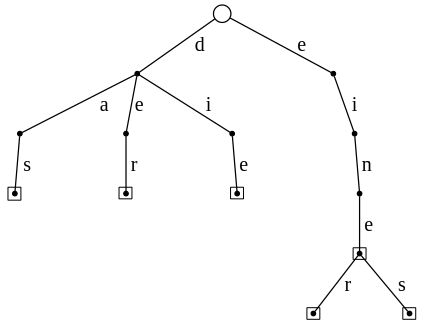
\includegraphics[scale=.5]{kap3Trie}
  \caption{Ein Trie, der die bestimmten und unbestimmten Artikel enthält.}
  \label{trie}
\end{figure}

In Abbildung \vref{trie} sehen wir ein einfaches Beispiel eines Tries. Das lässt sich zu Gunsten der Effizienz noch vereinfachen. Suffixbäume zum Beispiel sind Tries, die alle Suffixe eines Wortes speichern. Zur Konstruktion und Darstellung braucht man lineare Zeit im Verhältnis zur Wortlänge. Suffixbäume sind für DNA besonders gut geeignet. Suffixarrays vereinfachen diesen Ansatz noch.

\section{Prioritätswarteschlangen (priority queues)}
Eine weitere wichtige Datenstruktur, die wir im Folgenden immer wieder nutzen werden sind Prioritätswarteschlangen. Die üblichen Operationen auf einer Prioritätswarteschlange sind:
\begin{itemize}
  \item Streichen des Minimums (\texttt{delete-min}): finde und streiche das kleinste Objekt, also das Objekt mit der höchsten Priorität.
  \item Einfügen eines neuen Objekts (\texttt{insert}): hinzufügen eines neuen Objekts in die Warteschlange.
  \item Vermindere einen Schlüssel (\texttt{decrease-key}): vermindere den Wert eines Schlüssels, erhöhe also die Priorität eines Objekts.
\end{itemize}

Die Standarddatenstruktur dafür ist ein (binärer) Heap. Betrachten wir daher kurz die Laufzeiten der oben genannten Operationen auf einem einfachen und einem Fibonacci"=Heap:

\begin{center}
\begin{tabular}{lcc}
& Heap & \multirow{2}*{Fibonacci-Heaps}\\
& (schlechtester Fall) & \\\hline\hline
Streiche Minimum & $\Theta(\log n)$ & $\Theta(1)$ (amortisiert)\\
Einfügen & $\Theta(\log n)$ & $\mathcal{O}(\log n)$ (schlechtester Fall)\\
Vermindere Schlüssel & $\Theta(\log n)$ & $\Theta(1)$ (amortisiert)\\\hline\hline
\end{tabular}\\
\end{center}

$\mathcal{O}(\log n)$ Zeit ist auch mit Standarddatenstrukturen für Wörterbücher möglich, mit einem Heap jedoch einfacher zu implementieren.

\section{Union-Find (disjoint sets)}
Union-Find bezeichnet sowohl ein Problem, als auch eine Datenstruktur. Gegeben ist eine feste Menge $S$ von Daten (o.B.d.A. $S = \{1, \ldots, n\}$). Gesucht ist eine Partition von $S$ in disjunkte Teilmengen, also $S = S_1 \cupdot S_2 \cupdot \ldots \cupdot S_k$. Darauf aufbauend definieren wir zwei Operationen:
\begin{itemize}
  \item \texttt{Union}($S_i$, $S_j$): vereinige zwei Teilmengen in der Partition und erzeuge so eine neue Partition.
  \item \texttt{Find}($i$): finde die Teilmenge der Partition, die $i$ enthält.
\end{itemize}

Hierfür gibt es eine Reihe von Anwendungen, von denen wir einige beispielhaft benennen wollen, ehe wir die Datenstruktur genauer untersuchen:
\begin{itemize}
  \item Finden der Zusammenhangkomponente eines Graphen, insbesondere: finden minimaler Spannbäume.
  \item Segmentierung von Bildern in der Bildverarbeitung: Erkennen und Zerlegen des Bildes in Segmente, die zusammen gehören (z.B. weil sie die gleiche Farbe haben).
  \item Equivalence(X, Y) in Fortran: Prüfen, ob X und Y verschiedene Bezeichner für das Gleiche sind. Man schafft dabei auf der Menge aller Variablen eines Programms eine Partition.
\end{itemize}

\begin{figure}[htb]
  \centering
  \includegraphics[scale=.66]{kap3UnionFind1}
  \caption{Beispiel einer Union"=Find"=Struktur mit $S= \{1, \ldots, 10 \}$ und den Partitionen $\{1, 3, 5, 7, 9\}$ $\{2, 4\}$ $\{6, 8\}$ $\{10\}$.}
  \label{kap3UnionFind1}
\end{figure}

Welche Datenstruktur wählen wir, um das Union"=Find"=Problem effizient zu lösen? Die Datenstruktur ist ein Wald, das heißt eine Menge von Bäumen. Wir brauchen einen Baum pro Teilmenge $S_1, \ldots, S_k$. Jede davon hat einen Repräsentanten $a \in S_i$, der sich in der Wurzel des entsprechenden Baums befindet. Die Verweise innerhalb eines Baums verlaufen vom Kind zum Vater.

Die Operationen lassen sich auf dieser Datenstruktur nun leicht konkretisieren. \texttt{Find}($x$) sucht den Knoten $x$ und folgt dem Pfad aufwärts bis zur Wurzel. Der Repräsentant, der in der Wurzel steht wird als Ergebnis der Operation zurück gegeben. \texttt{Union}($S_i, S_j$) macht die Wurzel des Baums von $S_j$ zu einem Kind der Wurzel von $S_i$. Die Laufzeit für \texttt{Union} liegt natürlich in $\mathcal{O}(1)$ . Die Laufzeit von \texttt{Find} ist abhängig von der Höhe des Baumes $h$: $\mathcal{O}(h)$. Die Abbildung \vref{kap3UnionFindOp} veranschaulicht beide Operationen.

\begin{figure}[htb]
  \centering
  \subfloat[\label{kap3UnionFindOp1}]{\includegraphics[scale=0.5]{kap3UnionFindOp1}}\hspace{3em}
  \subfloat[\label{kap3UnionFindOp2}]{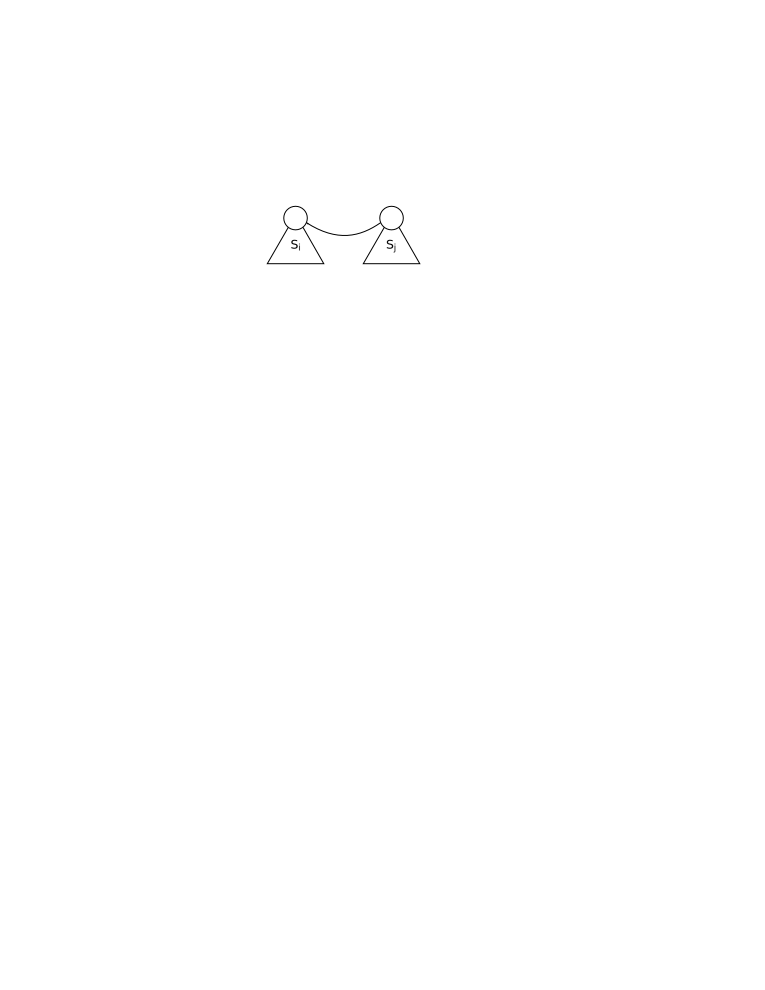
\includegraphics{kap3UnionFindOp2}}
  \caption{\subref{kap3UnionFindOp1} zeigt schematisch eine \texttt{Find}-Operation, Abbildung \subref{kap3UnionFindOp2} eine \texttt{Union}"=Operation.}
  \label{kap3UnionFindOp}
\end{figure}

Hat ein Baum die in Abbildung \vref{kap3UnionFindOp1} gezeigte Form, so hat \texttt{Find} eine Laufzeit von $\Theta(n)$. Dies lässt sich vermeiden, in dem die \texttt{Union}"=Operation immer den niedrigeren Baum an den Höheren hängt. Angenommen wir beginnen mit der Partition $\{1\}, \{2\}, \ldots, \{n\}$, und führen alle \texttt{Union}"=Operationen unter Beachtung des Höhenausgleichs durch, dann kann kein Baum die in Abbildung \vref{kap3UnionFindOp1} gezeigte Form annehmen.

\begin{Satz}
\hspace{\parindent}Führt man, beginnend mit der Partition $\{1\}, \ldots, \{n\}$, eine Folge von \texttt{Union}"=\texttt{Find}"=Operationen durch, wobei \texttt{Union} mit Höhenausgleich ausgeführt wird, so kostet \texttt{Union} $\mathcal{O}(1)$ und \texttt{Find} $\mathcal{O}(\log n)$ Zeit im schlechtesten Fall.
\end{Satz}

\begin{Bew}
\hspace{\parindent}Es ist zu zeigen, dass die Bäume nie höher werden als $\mathcal{O}(\log n)$. Dazu speichern wir mit jeder Wurzel noch die Höhe des Baums und zeigen durch Induktion über die Höhe $h$ eines Baums, dass jeder Baum $k \ge 2^h$ Knoten enthält.

Wir wählen als Induktionsanfang $h=0$. $2^h = 2^0 = 1$. Da ein Baum mit Höhe $0$ einen Knoten hat, stimmt die Induktionsvoraussetzung.

\begin{figure}[hbt]
  \centering
  \includegraphics[width=0.9\textwidth]{kap3UnionFindLfzBew}
  \caption{Eine \texttt{Union}"=Operation mit Höhenausgleich, bei der ein Baum mit $k=k_1 + k_2$ Knoten und Höhe $h= max(h_1, h_2 +1)$ entsteht.}
  \label{kap3UnionFindLfzBew}
\end{figure}

Es folgt der Induktionsschritt $h-1 \to h$: in Abbildung \vref{kap3UnionFindLfzBew} sehen wir die \texttt{Union}"=Operation, aus der der Baum $T$ der Höhe $h=max(h_1, h_2 +1)$ mit $k=k_1+k_2$ Knoten entstanden ist. Angenommen $h_1 > h_2$: offensichtlich gilt $k_1 + k_2 \ge k_1$ und nach Induktionsvoraussetzung $k_1 \ge 2^{h_1} = 2^h$, daher auch $k \ge 2^h$. Falls aber $h_1 = h_2$ ist, so gilt $k_1 + k_2 \ge 2^{h_1} + 2^{h_2} = 2 \cdot 2^{h_2} = 2^{h_2 +1} = 2^{h}$.
\end{Bew}

Geht es noch besser? Bereits den Höhenausgleich kann man als eine Art Heuristik ansehen. Die \textit{Pfadkompression} geht davon aus, dass man Knoten oft in den gleichen Teilbäumen sucht. Sucht man z.B. nach einem Knoten a, so sammelt die Pfadkompression alle Knoten und Teilbäume, die auf dem Weg von der Wurzel zum Knoten a liegen und hängt diese gesammelten Knoten und Teilbäume direkt an die Wurzel an. Ein nachfolgender Zugriff auf einen der Knoten aus diesem Teilbaum wird deutlich schneller erfolgen. Abbildung \vref{kap3Pfadkompression} veranschaulicht das vorgehen.

\begin{figure}[htb]
  \centering
  \includegraphics[scale=.5]{kap3Pfadkompression}
  \caption{Pfadkompression: alle Knoten auf dem Weg von der Wurzel zu Knoten a werden direkt an die Wurzel gehängt.}
  \label{kap3Pfadkompression}
\end{figure}

%Was kostet \texttt{Union}-\texttt{Find} mit Höhenausgleich und Pfadkompression?
%Im schlechtesten Fall: immer noch $\mathcal{O}(1)$ beziehungsweise $\mathcal{O}(\log n)$.
%Amortisiert, ausgehend von $1 \ldots n$, dann Folge von \texttt{Union}s und \texttt{Find}s $\rightarrow$ res. Wald.
%
%definieren Rang eines Konten $v$: ursprünglich $0$, wird um $1$ erhöht, bei allen \texttt{Union}-Operationen wo $v$ Wurzel wird und zwei Wurzeln mit gleichen Rängen vorliegen.
%Zeichnung 7
%Heuristik: \texttt{Union} gemäß Rang: Baum, dessen Wurzel den kleineren Rang hat, wird an den gehängt, dessen Wurzel den größeren Rang hat.

% vorlesung 11

%Pfadkompression: man durchläuft einen Weg vom Knoten zur Wurzel. Dabei sammelt man alle Teilbäume auf dem Weg auf und hängt sie an die Wurzel. Dadurch sollte die nächste \texttt{Find}-Operation schneller ablaufen.

\subsection{Amortisierte Laufzeitanalyse von Union"=Find mit Pfadkompression}
Die Analyse der Laufzeit von Union"=Find mit Pfadkompression wird eine der komplizierteren in dieser Vorlesung.

Wir nehmen an, dass am Anfang jedes Elemente aus $S$ eine einelementige Menge bildet. Dann wird eine Folge $\sigma$ von \texttt{Union"=Find}"=Operationen ausgeführt. \texttt{Union} arbeitet dabei gemäß des Rangs der Wurzelknoten, der beiden zu vereinigenden Bäume. Zu jedem Knoten wird dazu sein Rang gespeichert. Am Anfang haben alle Knoten Rang $0$, falls zwei Bäume vereinigt werden, deren Wurzeln den gleichen Rang $r$ haben, so erhält die neue Wurzel den Rang $r+1$.

\begin{figure}[htb]
  \centering
  \includegraphics[width=.75\textwidth]{kap3UnionByRang}
  \caption{Der Rang eines Wurzelknotens erhöht sich, wenn zwei Bäume vereinigt werden, deren Wurzelknoten gleichen Rang haben. Haben die Wurzelknoten unterschiedlichen Rang, ändern sich die Ränge nicht und der Wurzelknoten mit kleinerem Rang wird an den Wurzelknoten mit höherem Rang angefügt.}
  \label{kap3UnionByRang}
\end{figure}

In Abbildung \vref{kap3UnionByRang} sehen wir, wie Union nach Rang funktioniert und wie es sich auf den Rang eines Knotens auswirkt. Wir können nun einige Eigenschaften festhalten. Für alle Knoten $v$, Wurzel eines Unterbaums $T_v$ gilt:
\begin{enumerate}
  \item $T_v$ hat mindestens $2^{Rang(v)}$ Knoten.
  \item es gibt $\le \frac{n}{2^r}$ Knoten vom Rang $r$ (folgt direkt aus 1.)
  \item alle Ränge sind $\le \log n$ (folgt direkt aus 2.)
  \item Falls bei der Ausführung von $\sigma$ irgendwann $w$ Nachkomme von $v$ ist, dann ist der $Rang(w) < Rang(v)$. Denn jede Kante ist durch eine \texttt{Union}"=Operation entstanden, nach der $Rang(w) < Rang(v)$ (siehe Abbildung \vref{kap3UnionByRang}). \texttt{Find}"=Operationen ändern daran nichts.
\end{enumerate}

\begin{Bem}
  \hspace{\parindent}Für alle Knoten $v$, Wurzel eines Unterbaums $T_v$ gilt: Höhe $T_v \le Rang(v)$. Die Pfadkompression ändert daran nichts, da bei Pfadkompression zwar die Höhe geringer wird, der Rang sich jedoch nicht verändert.

  Auch für Union nach Rang ist der schlechteste Fall für \texttt{Find} $\mathcal{O}(\log n)$.
\end{Bem}

Zur amortisierten Analyse von Union"=Find mit Pfadkompression brauchen wir eine sehr schnell und eine sehr langsam wachsende Funktion. Wir definieren die Funktionen $F,G : \mathbb{N} \to \mathbb{N}$ wie folgt:

\begin{align*}
  F(0) &= 1 \\
  F(i) &= 2^{F(i-1)} \quad i=1, 2, 3, \ldots
\end{align*}

Bereits die ersten Werte der Funktion lassen ihr sehr starkes Wachstum erkennen.
\begin{center}
  \begin{tabular}{>{$}l<{$}|>{$}r<{$}|>{$}r<{$}|>{$}r<{$}|>{$}r<{$}|>{$}r<{$}|>{$}r<{$}|>{$}r<{$}}
    i & 0 & 1 & 2 & 3 & 4 & 5 & 6 \\\hline
    F(i) & 1 & 2 & 4 & 16 & 65536 & 2^{65536} & 2^{2^{65536}}
  \end{tabular}
\end{center}

Die Funktion $G$ ist eine sehr langsam wachsende Funktion. Wir definieren sie mit Bezug auf $F(n)$:
\[G(n) = min\{k \mid F(k) \ge n \}\]

Auch hier wollen wir exemplarisch einige Werte betrachten:
\begin{center}
  \begin{tabular}{>{$}l<{$}|>{$}r<{$}|>{$}r<{$}|>{$}r<{$}|>{$}r<{$}|>{$}r<{$}|>{$}r<{$}|>{$}r<{$}|>{$}r<{$}|>{$}r<{$}|>{$}r<{$}|>{$}r<{$}|>{$}r<{$}|>{$}r<{$}}
    n    & 0 & 1 & 2 & 3 & 4 & 5 & 6 & \ldots & 16 & \ldots & 65536 & \ldots & 2^{65536} -1 \\\hline
    G(n) & 0 & 0 & 1 & 2 & 2 & 3 & 3 & 3 & 3 & 4 & 4 & 5 & 5
  \end{tabular}
\end{center}

$G(n)$ heißt auch $\log^* n$ : wie oft muss man den Logarithmus auf $n$ anwenden damit man auf eine Zahl $\le 1$ kommt?

Wir hatten bereits angenommen, dass jedes Element aus $S$ am Anfang eine einelementige Menge bildet und dann eine Folge $\sigma$ von \texttt{Union"=Find}"=Operationen ausgeführt wird. Gehen wir weiter davon aus, dass $\sigma$ aus $\le n-1$ \texttt{Union}- und $m$ \texttt{Find}"=Operationen besteht. Wir teilen die Ränge der Knoten in Gruppen auf:

\begin{center}
  \begin{tabular}{l|>{$}r<{$}|>{$}r<{$}|>{$}r<{$}|>{$}r<{$}|>{$}r<{$}|>{$}r<{$}|>{$}r<{$}|>{$}r<{$}|>{$}r<{$}}
    $r$           & 0 & 1 & 2 & 3 & 4 & 5 & \ldots & 16 & \ldots\\\hline
    Gruppe $G(r)$ & 0 & 0 & 1 & 2 & 2 & 3 &      3 & 3 & \ldots
  \end{tabular}
\end{center}

Jedes \texttt{Union} kostet $\mathcal{O}(1)$ Zeit. \texttt{Find} kostet mehr, proportional zur Länge des Weges bis zur Wurzel. Im folgenden führen wir eine amortisierte Analyse mittels Buchhalter Methode durch. Für jeden Knoten $v$ auf dem Weg zur Wurzel entstehen konstante Kosten in Höhe von 1 \euro{}. Diese ordnen wir
\begin{enumerate}
  \item der \texttt{Find}"=Operation zu, falls $v$ die Wurzel ist oder der Vater $x$ von $v$ in einer anderen Ranggruppe als $v$ ist,
  \item ansonsten dem Knoten $v$ selbst zu.
\end{enumerate}

\begin{figure}[hbt]
  \centering
  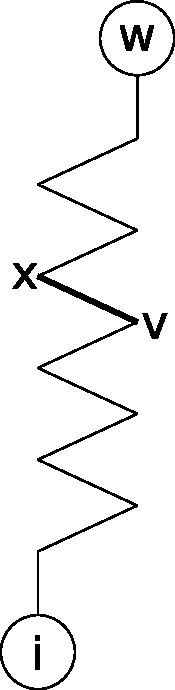
\includegraphics[scale=.4]{kap3DesZahlst}
  \caption{Die Ränge wachsen monton steigend von unten nach oben. Wenn sich die Ranggruppe von v und x unterscheidet, werden die Kosten der Find-Operation berechnet, sonst dem Knoten v.}
  \label{kap3DesZahlst}
\end{figure}

Keine \texttt{Find}"=Operation wird mit mehr als $G(n)$ Kosten belastet. Die Ränge sind laut der 4. Eigenschaft aufsteigend sortiert (monoton steigend). Die Ranggruppe kann sich höchstens $G(n)$ mal ändern, was der Anzahl der Ranggruppen entspricht. Eigentlich ändert sich die Ranggruppe sogar nur $G(\log{n})$ mal. Der Unterschied zwischen $G(n)$ und $G(\log n)$ ist höchstens $1$, da $G(\log n)$ den Logarithmus einmal mehr ausführt, als $G(n)$ dies bereits tut.

Wie viele Kosten fallen bei den Knoten selbst an? Betrachten wir Knoten $v$: Durch die Pfadkompression wird $v$ nach oben bewegt und wird Kind eines Vaters dessen Rang größer sein muss, als der seines bisherigen Vaters (wegen der monoton steigenden Ränge). Sei $g$ die Gruppe des Knotens $v$, also $g = G(Rang(v))$. Dann gibt es höchstens $F(g) - F(g-1)$ Ränge in der Gruppe g. Höchstens $F(g) - F(g-1)$ mal kann die Ranggruppe von $v$ der Ranggruppe seines Vaters entsprechen. Höchstens so oft kann also ein Knoten $v$ belastet werden.

Sei $N(g)$ die Anzahl der Knoten in Ranggruppe $g$. Wir können $N(g)$ bestimmen:
\[ N(g) \le \sum_{r=F(g-1)+1}^{F(g)}\frac{n}{2^r} \]
weil es laut der 2. Eigenschaft höchstens $\frac{n}{2^r}$ Knoten vom Rang $r$ gibt und es höchstens $F(g) - F(g-1)$ Ränge in Gruppe $g$ gibt. Wir können das umformen:
\begin{align*}
N(g) &\le \sum_{r=F(g-1)+1}^{F(g)}\frac{n}{2^r}\\
     &= \frac{n}{2^{F(g-1)+1}} (1 + \frac{1}{2} + \frac{1}{4} + \ldots)\\
     &\le \frac{n}{2^{F(g-1)}} \cdot \frac{1}{2} \cdot 2\\
     &= \frac{n}{2^{F(g-1)}} \\
     &= \frac{n}{F(g)}
\end{align*}

Es gibt also höchstens $\frac{n}{F(g)}$ Knoten in Ranggruppe $g$, die jeweils höchstens $F(g) - F(g-1) < F(g)$ mal belastet werden. Ranggruppe $g$ wird also maximal $\frac{n}{F(g)} \cdot F(g)$ mal belastet. Da es nicht mehr als $G(n)$ Ranggruppen gibt, liegen die Gesamtkosten aller Knoten in $\mathcal{O}(n \cdot G(n))$.

\begin{Satz}
  \hspace{\parindent}Ausgehend von einer Partition $S_i = \{ i \}$ mit $i = 1, \ldots , n$ wird eine Folge $\sigma$ ausgeführt, bestehend aus $\le n$ \texttt{Union}"=Operationen nach Rang und $m$ \texttt{Find}"=Operationen mit Pfadkompression. Die Gesamtlaufzeit von $\sigma$ liegt dann in $\mathcal{O}(n \log^*n + m \log^*n) = \mathcal{O}((n+m) \log^* n)$.
\end{Satz}

Aus diesem Satz folgt insbesondere, dass \texttt{Find} mit Pfadkompression eine amortisierte Laufzeit von $\mathcal{O}(\log^* n)$ hat.

Es sei noch angemerkt, dass es sogar noch schneller geht, auch wenn wir das im Folgenden nicht beweisen. Zunächst führen wir jedoch die \textit{Ackermann"=Funktion} ein: $A: \mathbb{N} \times \mathbb{N} \to \mathbb{N}$, definiert durch:
\begin{align*}
  A(0,0) &= 0\\
  A(i,0) &= 1 \quad i\ge 1 \\
  A(0,x) &= 2x \quad x \ge 0\\
  A(i+1, x) &= A(i, A(i+1, x-1))
\end{align*}

Daraus folgt:
\begin{align*}
  A(1,x) &= A(0, A(1, x-1)) = 2 \cdot A(1,x-1)\\
  A(2, x) &= A(1, A(2, x-1)) = 2^{A(2, x-1)}
\end{align*}

\begin{figure}[htb]
  \centering
  \begin{tabular}{l||>{$}r<{$}>{$}r<{$}>{$}r<{$}>{$}r<{$}>{$}r<{$}>{$}r<{$}}
%    \backslashbox[3em]{i}{x} & 0 & 1 & 2 & 3 & 4 & 5 \\\hline\hline
        & x=0 & x=1 & x=2 & x=3 & x=4 & x=5 \\\hline\hline
    $i=0$ & 0 & 2 & 4 & 6 & 8 & 10\\
    $i=1$ & 1 & 2 & 4 & 8 & 16 & 32\\
    $i=2$ & 1 & 2 & 4 & 16 & 65356 & \ldots\\
    $i=3$ & 1 & 2^2 & 2^{2^{2^{2}}} & \multicolumn{3}{l}{$2^{2^{\iddots^{2}}\big\} 65356}\quad\ldots$}
  \end{tabular}
  \caption{Einige Werte der Ackermann"=Funktion.}
  \label{AckermannWerte}
\end{figure}

$A(2,X)$ entspricht ungefähr $F(i)$. $A(z,4)$ wächst bereits viel stärker als $F(i)$.

Es gibt auch eine Funktion, die \textit{inverse Ackermann"=Funktion} genannt wird:
\[ \alpha(m, n) = min \{z \ge 1 \mid A(z, 4 \cdot \lceil\frac{m}{n}\rceil) > \log n\} \]

\begin{Satz}
  \hspace{\parindent}Ausgehend von einer Partition $S_i = \{ i \}$ mit $i = 1, \ldots , n$ wird eine Folge $\sigma$ ausgeführt, bestehend aus $\le n$ \texttt{Union}"=Operationen nach Rang und $m$ \texttt{Find}"=Operationen mit Pfadkompression. Die Gesamtlaufzeit von $\sigma$ liegt dann in $\mathcal{O}(m \cdot \alpha(m,n))$.
\end{Satz}

Den Beweis führen wir hier nicht.
